\section{Setup}
\label{sec:setup}
\subsection{Data, the label error and three evaluation views}
Waterbirds has 4,795 training, 1,199 validation and 5,794 test images. A group is a pair (bird class, background); the test groups landbird-on-land, landbird-on-water, waterbird-on-land and waterbird-on-water contain 2,255, 2,255, 642 and 642 images. WGA is the minimum of the four group accuracies, computed per backbone and then averaged.

The generating script \cite{sagawa2020code} labels a CUB species as a waterbird if its lower-cased name contains any keyword from a list of seabirds and waterfowl, one of which is \texttt{tern}. The substring also occurs in \texttt{eastern} and \texttt{western}. Three species match no intended keyword and are labelled waterbird only through this match: 021 Eastern Towhee, 088 Western Meadowlark and 102 Western Wood-Pewee. Western Grebe and Western Gull also contain \texttt{tern} but are waterbirds through \texttt{grebe} and \texttt{gull}; a pass over all 46 waterbird-labelled species finds no other case. The affected images are 72 training, 18 validation (11 of the 133 waterbird-on-land and 7 of the 133 waterbird-on-water images) and 90 test images (43 and 47 of the two waterbird test groups of 642).

We score every prediction in three views of the test set: \emph{official} labels; \emph{corrected} labels, in which the 90 images are relabelled landbird and move to the landbird groups; and the \emph{clean} subset of 5,704 images that remains after removing the 90 images, which changes no label. We treat the clean subset as the primary corrected view because it involves no relabelling; the corrected view gives nearly identical differences. Unless stated otherwise, heads and calibrators are fitted on the official validation labels and backbones on the official training labels.

\subsection{Backbones and heads}
We use seven ResNet-50 backbones saved from earlier runs: five standard ERM backbones (seeds 0--4, 100 epochs) and two ERM$^*$ backbones (seeds 0--1, 400 epochs with augmentation), reported separately because they are different recipes. All heads act on frozen 2,048-dimensional features of the validation and test images.

\textbf{DPE.} Fifteen two-prototype distance-based heads are trained in sequence on group-balanced subsets of the validation features \cite{to2025dpe}: 20 epochs per head, batch size 256, learning rate $10^{-3}$, momentum 0.9, entropic scale 30, covariance penalty $5\times10^5$ (decaying by stage for standard ERM, constant for ERM$^*$ as in the preserved recipes). For standard ERM each head keeps the epoch with the highest WGA on its own training pool. The prediction averages the head probabilities. \emph{Full-validation DPE}, fitted on all 1,199 images, is the reference throughout.

\textbf{DFR-lite.} As a second validation-label method we fit group-weighted L1-penalised logistic regression on standardised features of the validation set, choosing $C\in\{0.01,0.03,0.1,0.3,1\}$ by five-fold validation WGA. It shares DFR's inputs \cite{kirichenko2023dfr} but not its repeated balanced subsampling, so it is not a faithful DFR.

\subsection{Post-hoc procedures}
\textbf{Combiners on held-out images.} Heads are trained on 720 validation images and a combiner on the remaining 479 (group-stratified). The combiners are an affine map $\sigma(a s+b)$ of the ensemble score $s=\mathrm{logit}\,\bar q$ and a \emph{linear residual}, which adds a linear function of the 15 head scores to that map. Both are compared with the uniform ensemble of the same 720-image heads and with full-validation DPE. An earlier fixed-setting study on three partitions also covered weighting rules, logistic and MLP combiners and prototype-level weights (Sect.~\ref{sec:agg}).

\textbf{Cross-fitting.} Five 15-head ensembles are each trained on four fifths of the validation set. An affine map is fitted on the 1,199 out-of-fold scores and applied to each fold ensemble before averaging, so no image is held back from head training. Variants and controls: the uncalibrated fold ensemble; an offset-only map ($a=1$); the out-of-fold map applied instead to full-validation DPE; an exact WGA threshold on the averaged score; and a 75-head bag of five full-validation ensembles, which has as many heads as cross-fitting but no out-of-fold scores. Maps minimise group-averaged or worst-group cross-entropy with penalty $\lambda[(a-1)^2+b^2]$, $\lambda\in\{0.01,0.1\}$, using 400 full-batch Adam steps.

\textbf{Validation labels.} Separately, full-validation DPE (five head seeds per backbone) and DFR-lite are refitted after relabelling the 18 affected validation images as landbirds, or after dropping them, and compared with the refit on official labels.

\subsection{Protocol and stages}
\textbf{Validation-only selection.} For each procedure, one of four settings (group-averaged or worst-group loss, $\lambda\in\{0.01,0.1\}$) is chosen by the lowest group-balanced negative log-likelihood (primary rule) or the highest WGA (secondary) in an inner five-fold cross-validation. The inner cross-validation is strictly nested: every head ensemble and calibrator used to score an inner fold is refitted without that fold, and the score is that of the complete procedure applied at test time. The whole pipeline, including head-training seeds, fold assignments and the 720/479 partition, is repeated for ten split seeds, and full-validation DPE is retrained with the same seeds, so every comparison is paired within a cell. The fixed setting (group-averaged loss, $\lambda=0.1$) is reported as well.

\textbf{Stages.} The study has three stages that differ in their independence from the test set. (i) Exploratory development on the seven saved backbones, during which test results were inspected and the candidate procedures were chosen. (ii) The strictly nested rerun above, in which every setting was chosen on validation data; it was first scored on official labels, and then re-scored on corrected labels and the clean subset by rebuilding each prediction from its saved checkpoints, without refitting or reselecting anything (every rebuilt prediction reproduces its recorded official-label WGA exactly). (iii) A replication of the validation-label effect on four fresh backbones, with the contrast declared before the run. Fresh backbones replicate training randomness; they are not new test images.

\textbf{Statistics.} Differences are paired per backbone, averaged over seeds within a backbone, and reported with pointwise 95\% $t$ intervals over the five standard-ERM backbones. With two ERM$^*$ backbones we report means only. Seeds, folds and partitions are repeats within a backbone and are not counted as independent evidence; intervals describe variation over backbones on this one dataset. Over ten split seeds, full-validation DPE has a within-backbone SD of 0.40\pp{} (standard ERM) and 0.33\pp{} (ERM$^*$).

\section{Results}
\label{sec:results}
\subsection{Reproduction}
Table~\ref{tab:repro} compares our full-validation DPE with the published numbers. Our standard-ERM DPE is 1.1--1.4\pp{} below the reported 91.0\%; ERM$^*$ matches. To check whether the gap comes from our implementation, we ran the authors' code end to end on two fresh ERM backbones. The backbones match the reported ERM accuracy (69.3\% against 69.1\%), and DPE reaches 89.4\% and 86.5\%. The official pipeline is therefore also below 91.0\% in our hands, and our results should be read relative to our own full-validation DPE.

\begin{table}[t]
\centering\small
\caption{Reproduction of full-validation DPE (test WGA, \%, official labels).}
\label{tab:repro}
\begin{tabular}{@{}llrr@{}}
\toprule
Recipe & Run & DPE & Reported \cite{to2025dpe}\\\midrule
ERM & ours, 5 backbones, saved heads & 89.60 & 91.0\\
ERM & ours, 5 backbones, mean over 10 head seeds & 89.88 & 91.0\\
ERM & authors' code, fresh backbones (seeds 5, 6) & 89.41, 86.47 & 91.0\\
ERM$^*$ & ours, 2 backbones, saved heads & 94.08 & 94.1\\
ERM$^*$ & ours, 2 backbones, mean over 10 head seeds & 93.88 & 94.1\\
\bottomrule
\end{tabular}
\end{table}

\subsection{Post-hoc procedures: lost on official labels, gained on correct ones}
Fig.~\ref{fig:levers} and Table~\ref{tab:main} give the main result. On official labels, no procedure with validation-selected settings beats full-validation DPE: cross-fitted recalibration is $-0.17$\pp{} ($[-0.33,-0.02]$), the out-of-fold map applied to full-validation DPE $-0.58$\pp{} and the linear residual $-0.86$\pp. On the clean subset the same predictions are ahead on every standard-ERM backbone: $+1.11$\pp{} ($[+0.67,+1.56]$), $+1.39$\pp{} ($[+1.13,+1.65]$) and $+1.74$\pp{} ($[+1.45,+2.03]$). Relabelling instead of removing the 90 images gives $+1.21$, $+1.44$ and $+1.75$\pp. The secondary WGA selection rule gives the same picture. On ERM$^*$ the gains on the clean subset are smaller: $+0.88$\pp{} for cross-fitted recalibration and $+0.73$\pp{} for the out-of-fold map, and $+0.08$\pp{} for the linear residual.

\begin{figure}[t]
\centering\resizebox{\linewidth}{!}{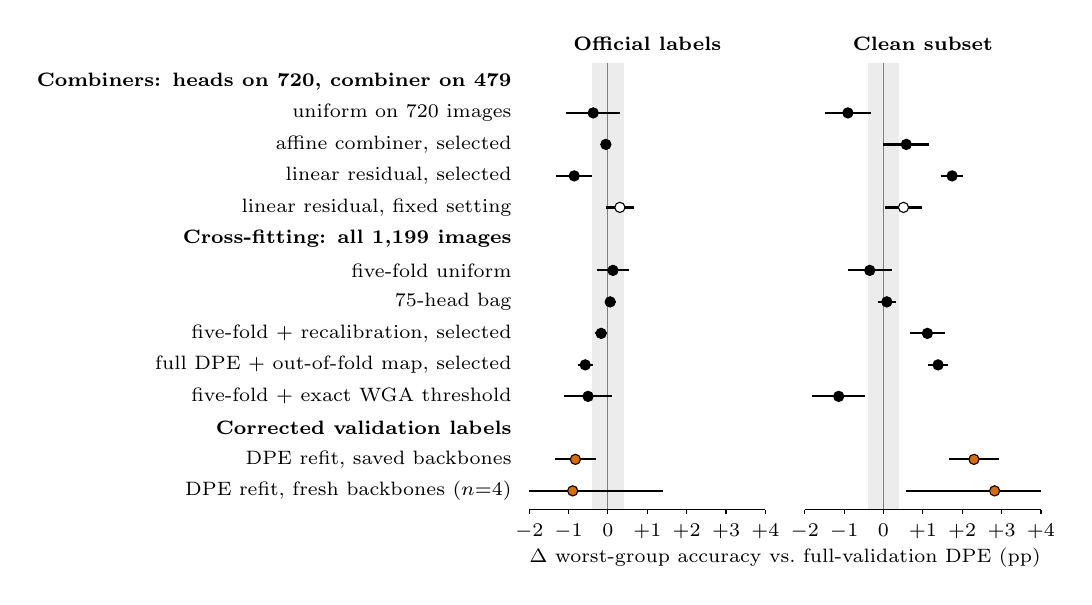
\begin{tikzpicture}[font=\scriptsize,y=0.40cm]
\fill[gray!15] (0.797,0.6) rectangle (1.203,-13.60);
\draw[gray] (1.000,0.6) -- (1.000,-13.60);
\draw (0.000,-13.60) -- (3.000,-13.60);
\draw (0.000,-13.60) -- ++(0,-0.15) node[below]{$-2$};
\draw (0.500,-13.60) -- ++(0,-0.15) node[below]{$-1$};
\draw (1.000,-13.60) -- ++(0,-0.15) node[below]{$0$};
\draw (1.500,-13.60) -- ++(0,-0.15) node[below]{$+1$};
\draw (2.000,-13.60) -- ++(0,-0.15) node[below]{$+2$};
\draw (2.500,-13.60) -- ++(0,-0.15) node[below]{$+3$};
\draw (3.000,-13.60) -- ++(0,-0.15) node[below]{$+4$};
\node[font=\scriptsize\bfseries] at (1.500,1.2) {Official labels};
\draw[thick] (0.469,-1) -- (1.157,-1);
\node[draw,circle,fill=black,inner sep=1.3pt] at (0.813,-1) {};
\draw[thick] (0.916,-2) -- (1.032,-2);
\node[draw,circle,fill=black,inner sep=1.3pt] at (0.974,-2) {};
\draw[thick] (0.339,-3) -- (0.804,-3);
\node[draw,circle,fill=black,inner sep=1.3pt] at (0.572,-3) {};
\draw[thick] (0.974,-4) -- (1.329,-4);
\node[draw,circle,fill=white,inner sep=1.3pt] at (1.152,-4) {};
\draw[thick] (0.860,-6) -- (1.267,-6);
\node[draw,circle,fill=black,inner sep=1.3pt] at (1.064,-6) {};
\draw[thick] (0.960,-7) -- (1.099,-7);
\node[draw,circle,fill=black,inner sep=1.3pt] at (1.029,-7) {};
\draw[thick] (0.836,-8) -- (0.992,-8);
\node[draw,circle,fill=black,inner sep=1.3pt] at (0.914,-8) {};
\draw[thick] (0.616,-9) -- (0.807,-9);
\node[draw,circle,fill=black,inner sep=1.3pt] at (0.712,-9) {};
\draw[thick] (0.443,-10) -- (1.053,-10);
\node[draw,circle,fill=black,inner sep=1.3pt] at (0.748,-10) {};
\draw[thick] (0.332,-12) -- (0.843,-12);
\node[draw,circle,fill=orange!85!black,inner sep=1.3pt] at (0.587,-12) {};
\draw[thick] (0.000,-13) -- (1.698,-13);
\node[draw,circle,fill=orange!85!black,inner sep=1.3pt] at (0.553,-13) {};
\fill[gray!15] (4.298,0.6) rectangle (4.703,-13.60);
\draw[gray] (4.500,0.6) -- (4.500,-13.60);
\draw (3.500,-13.60) -- (6.500,-13.60);
\draw (3.500,-13.60) -- ++(0,-0.15) node[below]{$-2$};
\draw (4.000,-13.60) -- ++(0,-0.15) node[below]{$-1$};
\draw (4.500,-13.60) -- ++(0,-0.15) node[below]{$0$};
\draw (5.000,-13.60) -- ++(0,-0.15) node[below]{$+1$};
\draw (5.500,-13.60) -- ++(0,-0.15) node[below]{$+2$};
\draw (6.000,-13.60) -- ++(0,-0.15) node[below]{$+3$};
\draw (6.500,-13.60) -- ++(0,-0.15) node[below]{$+4$};
\node[font=\scriptsize\bfseries] at (5.000,1.2) {Clean subset};
\draw[thick] (3.756,-1) -- (4.340,-1);
\node[draw,circle,fill=black,inner sep=1.3pt] at (4.048,-1) {};
\draw[thick] (4.495,-2) -- (5.082,-2);
\node[draw,circle,fill=black,inner sep=1.3pt] at (4.789,-2) {};
\draw[thick] (5.226,-3) -- (5.515,-3);
\node[draw,circle,fill=black,inner sep=1.3pt] at (5.371,-3) {};
\draw[thick] (4.517,-4) -- (4.991,-4);
\node[draw,circle,fill=white,inner sep=1.3pt] at (4.754,-4) {};
\draw[thick] (4.049,-6) -- (4.602,-6);
\node[draw,circle,fill=black,inner sep=1.3pt] at (4.325,-6) {};
\draw[thick] (4.424,-7) -- (4.659,-7);
\node[draw,circle,fill=black,inner sep=1.3pt] at (4.542,-7) {};
\draw[thick] (4.834,-8) -- (5.281,-8);
\node[draw,circle,fill=black,inner sep=1.3pt] at (5.057,-8) {};
\draw[thick] (5.063,-9) -- (5.323,-9);
\node[draw,circle,fill=black,inner sep=1.3pt] at (5.193,-9) {};
\draw[thick] (3.594,-10) -- (4.269,-10);
\node[draw,circle,fill=black,inner sep=1.3pt] at (3.931,-10) {};
\draw[thick] (5.327,-12) -- (5.970,-12);
\node[draw,circle,fill=orange!85!black,inner sep=1.3pt] at (5.649,-12) {};
\draw[thick] (4.788,-13) -- (6.500,-13);
\node[draw,circle,fill=orange!85!black,inner sep=1.3pt] at (5.911,-13) {};
\node[below] at (3.250,-14.50) {$\Delta$ worst-group accuracy vs.\ full-validation DPE (pp)};
\node[anchor=east,font=\scriptsize\bfseries] at (-0.1,0) {Combiners: heads on 720, combiner on 479};
\node[anchor=east] at (-0.1,-1) {uniform on 720 images};
\node[anchor=east] at (-0.1,-2) {affine combiner, selected};
\node[anchor=east] at (-0.1,-3) {linear residual, selected};
\node[anchor=east] at (-0.1,-4) {linear residual, fixed setting};
\node[anchor=east,font=\scriptsize\bfseries] at (-0.1,-5) {Cross-fitting: all 1,199 images};
\node[anchor=east] at (-0.1,-6) {five-fold uniform};
\node[anchor=east] at (-0.1,-7) {75-head bag};
\node[anchor=east] at (-0.1,-8) {five-fold + recalibration, selected};
\node[anchor=east] at (-0.1,-9) {full DPE + out-of-fold map, selected};
\node[anchor=east] at (-0.1,-10) {five-fold + exact WGA threshold};
\node[anchor=east,font=\scriptsize\bfseries] at (-0.1,-11) {Corrected validation labels};
\node[anchor=east] at (-0.1,-12) {DPE refit, saved backbones};
\node[anchor=east] at (-0.1,-13) {DPE refit, fresh backbones ($n{=}4$)};
\end{tikzpicture}
}
\caption{Test WGA relative to full-validation DPE retrained with the same seeds, standard ERM, mean and 95\% interval over five backbones. Left: official labels. Right: the 5,704 correctly labelled test images (the 90 images of the three mislabelled species removed). Black: settings chosen on validation data (ten split seeds, strictly nested); open: fixed setting; orange: DPE refitted on corrected validation labels against the official-label refit (saved backbones; fresh backbones with the authors' code, $n=4$). Shaded: $\pm$ one head-seed SD.}
\label{fig:levers}
\end{figure}

\begin{table}[t]
\centering\small
\caption{Test WGA difference (pp) against full-validation DPE retrained with the same seeds, in three views of the test set: official labels, corrected labels and the clean subset (90 images removed). Ten split seeds, strictly nested; interval: 95\% over five standard-ERM backbones; ``$+$'': backbones with a positive difference. ERM$^*$: clean subset, mean of two backbones.}
\label{tab:main}
\resizebox{\linewidth}{!}{\begin{tabular}{@{}lrrrrr@{}}
\toprule
& \multicolumn{4}{c}{Standard ERM ($n=5$)} & ERM$^*$\\
Procedure & Official & Corrected & Clean & 95\% interval (clean), $+$ & Clean\\\midrule
Full-validation DPE (WGA, \%) & 89.88 & 90.49 & 90.56 & & 94.41\\\midrule
Cross-fit + recalibration, selected (NLL) & $-0.17$ & $+1.21$ & $+1.11$ & $[+0.67,+1.56]$, 5/5 & $+0.88$\\
Cross-fit + recalibration, selected (WGA) & $-0.08$ & $+1.11$ & $+1.02$ & $[+0.65,+1.39]$, 5/5 & $+0.84$\\
Cross-fit + recalibration, fixed setting & $+0.17$ & $+0.63$ & $+0.55$ & $[+0.06,+1.03]$, 5/5 & $+0.55$\\
Full DPE + out-of-fold map, selected (NLL) & $-0.58$ & $+1.44$ & $+1.39$ & $[+1.13,+1.65]$, 5/5 & $+0.73$\\
720/479 linear residual, selected (NLL) & $-0.86$ & $+1.75$ & $+1.74$ & $[+1.45,+2.03]$, 5/5 & $+0.08$\\
720/479 linear residual, fixed setting & $+0.30$ & $+0.51$ & $+0.51$ & $[+0.03,+0.98]$, 5/5 & $-0.41$\\
720/479 affine, selected (NLL) & $-0.05$ & $+0.65$ & $+0.58$ & $[-0.01,+1.16]$, 4/5 & $+0.40$\\\midrule
720/479 uniform (heads on 720 images only) & $-0.37$ & $-0.87$ & $-0.90$ & $[-1.49,-0.32]$, 0/5 & $-0.50$\\
Cross-fit, uniform & $+0.13$ & $-0.29$ & $-0.35$ & $[-0.90,+0.20]$, 1/5 & $+0.04$\\
75-head bag (five full-validation ensembles) & $+0.06$ & $+0.09$ & $+0.08$ & $[-0.15,+0.32]$, 3/5 & $-0.05$\\
Cross-fit, exact WGA threshold & $-0.50$ & $-1.10$ & $-1.14$ & $[-1.81,-0.46]$, 0/5 & $-0.85$\\
Full DPE, exact WGA threshold & $-0.31$ & $-0.77$ & $-0.73$ & $[-1.08,-0.37]$, 0/5 & $-0.81$\\
\bottomrule
\end{tabular}}
\end{table}

\subsection{Why official labels hide the gains: the wrong worst group}
Table~\ref{tab:groups} breaks the result down by group. With official labels, waterbird-on-land is the lowest group of full-validation DPE (90.0\%), but most of its errors are on the 43 mislabelled images: DPE predicts landbird, correctly, for 78 of the 90 mislabelled test images, and the official labels count these as errors. On the clean subset, waterbird-on-land rises to 95.5\%, waterbird-on-water to 98.2\%, and the worst group is landbird-on-water (90.6\%). The post-hoc procedures raise landbird-on-water, the true worst group, by 1.1--2.2\pp{}, at a cost to groups that remain well above it. On official labels this gain is invisible: the two waterbird groups, which hold the 90 mislabelled images, are artificially low and set the minimum (waterbird-on-water at 89.2\% for the linear residual), so a method that trades waterbird accuracy for landbird-on-water accuracy is scored as worse.

\begin{table}[t]
\centering\small
\caption{Per-group test accuracy (\%) of full-validation DPE and three post-hoc procedures on official labels and on the clean subset (90 mislabelled images removed). Standard ERM, mean over ten split seeds and five backbones; the lowest group in each row is in bold.}
\label{tab:groups}
\resizebox{\linewidth}{!}{\begin{tabular}{@{}llrrrr@{}}
\toprule
Test view & Procedure & Land/land & Land/water & Water/land & Water/water\\\midrule
Official & Full-validation DPE & 94.13 & 90.56 & \textbf{90.00} & 91.95\\
Official & Cross-fit + recalibration, selected & 93.42 & 91.67 & \textbf{89.72} & 90.87\\
Official & Full DPE + out-of-fold map, selected & 95.12 & 91.94 & \textbf{89.31} & 91.19\\
Official & 720/479 linear residual, selected & 93.83 & 92.75 & 90.08 & \textbf{89.19}\\
\midrule
Clean & Full-validation DPE & 94.13 & \textbf{90.56} & 95.54 & 98.20\\
Clean & Cross-fit + recalibration, selected & 93.42 & \textbf{91.67} & 95.32 & 97.49\\
Clean & Full DPE + out-of-fold map, selected & 95.12 & \textbf{91.94} & 94.89 & 97.70\\
Clean & 720/479 linear residual, selected & 93.83 & \textbf{92.75} & 95.52 & 95.53\\
\bottomrule
\end{tabular}}
\end{table}

\subsection{What the gains are made of}
\textbf{Head information beyond recalibration.} On the clean subset the linear residual beats the affine map fitted on the same 720-image heads by $+1.16$\pp{} ($[+0.79,+1.54]$, 5/5) with selected settings and by $+0.50$\pp{} ($[+0.27,+0.73]$, 5/5) at the fixed setting, so a linear function of the individual head scores carries information beyond any scalar map of the ensemble score. On official labels the same comparison is $-0.81$ and $+0.15$\pp.

\textbf{Recalibration acts through its offset.} Cross-fitted affine recalibration and the offset-only control ($a=1$) are within $0.1$\pp{} of each other at every setting on official labels, and with selected settings the difference on the clean subset is $-0.07$\pp{} ($[-0.16,+0.02]$). This is an empirical finding for our maps, which are applied to each fold ensemble before averaging, not an identity: the gain comes from moving the decision boundary of the ensemble, not from changing its slope. Selection matters for how far the boundary moves: the likelihood rule chose the weaker penalty $\lambda=0.01$ in all cells, which looks worse than the fixed setting on official labels but is better on the clean subset.

\textbf{Holding images back costs, cross-fitting avoids the cost.} Training the heads on 720 instead of 1,199 images costs $-0.90$\pp{} on the clean subset ($[-1.49,-0.32]$, 0/5); the linear residual more than recovers it ($+2.65$\pp{} over the 720-image ensemble). Cross-fitting avoids the cost, but without recalibration it brings no clear benefit: uniform cross-fitting is $-0.35$\pp{} ($[-0.90,+0.20]$) relative to full-validation DPE and $-0.43$\pp{} ($[-0.85,-0.01]$) relative to the 75-head bag.

\textbf{Thresholds tuned for WGA do not transfer.} An exact search for the threshold that maximises out-of-fold WGA raises fitted validation WGA but lowers test WGA in every view ($-1.14$\pp{} on the clean subset for cross-fitting). One plausible reason is that the search maximises WGA on validation labels that contain the same error, so it tunes the threshold to the wrong worst group; the likelihood criterion, which averages over all images of each group, is less sensitive to this.

\subsection{Aggregation over partitions (official labels)}
\label{sec:agg}
The broader exploratory study of stage (i) evaluated 840 fixed aggregation predictors per recipe on three 720/479 partitions, scored on official labels only. Table~\ref{tab:agg} lists the strongest. Against the uniform ensemble of the same heads, learned aggregators improve WGA on most partitions, but the matched ensemble itself moves by 0.9\pp{} between partitions, so the comparison with full-validation DPE depends on the partition: prototype importance falls from $+0.96$ to $-1.08$\pp, and the dropout MLP's gain over its matched ensemble falls from $+0.62$ to $+0.28$ and $-0.14$\pp. Global weighting rules barely act: the 12 power rules change $+0.03$ to $+0.12$\pp. The best of the 840 predictors, picked on the test set, is $+1.06$\pp{} ahead of full-validation DPE; it is a test-selected reference within this grid, not an achievable result, and the validation selectors of stage (ii) searched only the affine and linear-residual families.

\begin{table}[t]
\centering\small
\caption{Fixed-setting aggregators of the exploratory study (heads on 720 images, aggregator on 479): test WGA difference (pp, official labels) against the matched uniform ensemble and against full-validation DPE (saved heads, 89.60\%) on three partitions. Standard ERM, mean over five backbones; ERM$^*$: mean over partitions and two backbones.}
\label{tab:agg}
\resizebox{\linewidth}{!}{\begin{tabular}{@{}lrrrrrrr@{}}
\toprule
& \multicolumn{3}{c}{vs.\ matched ensemble} & \multicolumn{3}{c}{vs.\ full-validation DPE} & ERM$^*$\\
Aggregator & P0 & P1 & P2 & P0 & P1 & P2 & vs.\ full\\\midrule
Matched uniform ensemble (720 images) & -- & -- & -- & $-0.36$ & $+0.53$ & $+0.11$ & $-0.48$\\
Affine map of the ensemble score & $+0.53$ & $+0.18$ & $+0.20$ & $+0.16$ & $+0.70$ & $+0.31$ & $-0.22$\\
Linear residual on head scores & $+1.11$ & $+0.40$ & $+0.56$ & $+0.75$ & $+0.93$ & $+0.67$ & $-0.65$\\
Prototype importance & $+1.32$ & $-0.02$ & $-1.19$ & $+0.96$ & $+0.51$ & $-1.08$ & $-0.25$\\
\bottomrule
\end{tabular}}
\end{table}

\subsection{Correcting the validation labels}
Refitting DPE after relabelling the 18 affected validation images raises WGA on the clean subset by $+2.30$\pp{} ($[+1.65,+2.94]$, 5/5) and on corrected labels by $+2.48$\pp{} ($[+1.80,+3.15]$); dropping the 18 images instead gives $+2.27$\pp{} on the clean subset (Table~\ref{tab:labels}). On ERM$^*$ the gains on corrected labels are $+2.12$ and $+2.08$\pp. DFR-lite gains on standard ERM ($+1.40$\pp{} on the clean subset, $[+1.07,+1.74]$) but not on ERM$^*$. On official labels the same fix again looks harmful ($-0.83$\pp{} for DPE): the refitted models call more of the 90 mislabelled test images landbird (86 instead of 78 on average). Because relabelling and dropping give nearly the same gain, much of the effect may come from removing the wrong labels' influence on the group-balanced head training rather than from the corrected labels themselves; a matched random-removal control would separate the two.

\begin{table}[t]
\centering\small
\caption{Test WGA (\%) after fitting on official, corrected or reduced (drop) validation labels, on official labels and on the clean subset. Means over five head seeds (DPE) and over backbones. $\Delta$: paired difference to the official-label fit on the clean subset, 95\% interval over five standard-ERM backbones.}
\label{tab:labels}
\resizebox{\linewidth}{!}{\begin{tabular}{@{}llrrrrr@{}}
\toprule
& & \multicolumn{3}{c}{Standard ERM ($n=5$)} & \multicolumn{2}{c}{ERM$^*$ ($n=2$)}\\
Method & Fit labels & Official & Clean & $\Delta$ clean & Official & Clean\\\midrule
DPE & official & 89.89 & 90.42 & -- & 93.88 & 94.25\\
DPE & corrected & 89.07 & \textbf{92.72} & $+2.30$ $[+1.65,+2.94]$ & 92.74 & \textbf{95.84}\\
DPE & drop & 89.07 & 92.69 & $+2.27$ $[+1.72,+2.82]$ & 93.16 & 95.87\\\midrule
DFR-lite & official & 88.62 & 89.09 & -- & 92.68 & 94.97\\
DFR-lite & corrected & 86.70 & 90.49 & $+1.40$ $[+1.07,+1.74]$ & 88.94 & 94.15\\
DFR-lite & drop & 86.54 & 90.38 & $+1.29$ $[+0.94,+1.63]$ & 89.25 & 94.17\\
\bottomrule
\end{tabular}}
\end{table}

\textbf{Replication on fresh backbones.} We repeated this study on four fresh ERM backbones (seeds 5--8) trained with the authors' SubpopBench code, two of which are the backbones of Table~\ref{tab:repro}, with the authors' unmodified DPE and three head seeds each. Training labels and DPE validation labels (official or corrected) were crossed, and the primary contrast was fixed in the analysis script before the run. All 48 jobs completed. Correcting the validation labels raises WGA by $+2.82$\pp{} on the clean subset ($[+0.58,+5.07]$) and by $+3.04$\pp{} on corrected labels ($[+0.59,+5.48]$, all four backbones positive), and is $-0.89$\pp{} on official labels (Table~\ref{tab:replication}). Correcting the 72 training labels as well adds $+0.28$\pp{} ($[-0.40,+0.96]$) on corrected labels.

\begin{table}[t]
\centering\small
\caption{Replication on four fresh ERM backbones with the authors' code (seeds 5--8, three head seeds each): test WGA (\%) by training and validation label set, and the declared primary contrast.}
\label{tab:replication}
\begin{tabular}{@{}llrr@{}}
\toprule
Backbone labels & DPE validation labels & Official test & Corrected test\\\midrule
official & official & 88.11 & 88.40\\
official & corrected & 87.21 & \textbf{91.44}\\
corrected & official & 88.94 & 89.45\\
corrected & corrected & 86.94 & \textbf{91.72}\\\midrule
\multicolumn{2}{@{}l}{Primary: fix validation labels ($\Delta$, 95\% interval)} & $-0.89$ & $+3.04$ $[+0.59,+5.48]$\\
\bottomrule
\end{tabular}
\end{table}

\section{Discussion}
\textbf{What the evidence supports.} Under the tested conditions, post-hoc procedures that use DPE's validation set more carefully do improve its worst-group accuracy, by 1.1--1.7\pp{} on standard ERM, once the evaluation does not count correct predictions on mislabelled images as errors. A linear combiner of head scores helps beyond recalibration, and cross-fitting allows recalibration without holding images back. These gains were invisible, even reversed, on the official labels, because 90 mislabelled test images determine which group is worst. Correcting the validation labels is a separate and larger lever in our measurements. We did not test whether the post-hoc procedures add to corrected validation labels; the levers may be complementary.

\textbf{Recommendations.} For last-layer methods evaluated on Waterbirds: (i) report WGA on the clean subset or on corrected labels alongside the official labels, together with per-group accuracies; (ii) compare a stacked or recalibrated variant both with the ensemble of the same heads and with the method fitted on all validation images; (iii) choose settings on validation data over several split seeds; and (iv) be wary of validation criteria based on WGA alone while the validation labels contain the same error.

\textbf{Limitations.} The study covers one dataset and one method family, with five standard-ERM and two ERM$^*$ backbones; the gains are smaller on ERM$^*$, and the linear residual does not help there. The candidate procedures were chosen during exploratory development in which the test set was inspected, and the scoring on the clean subset was added after the nested run, although nothing was refitted or reselected for it. The evaluation views differ only in three species; other possible label issues, such as images that show several birds \cite{asgari2022masktune}, remain. DFR-lite is not a faithful DFR. Our standard-ERM DPE is below the published figure, as is the authors' code in our hands. Intervals are pointwise and over backbones only. Improved WGA does not show that a model relies less on backgrounds.

\section{Conclusion}
Post-hoc calibration and aggregation of diverse prototypical ensembles appear useless on the official Waterbirds test labels and are clearly useful on its correctly labelled images. The difference comes from a known error: three landbird species are labelled waterbird because ``tern'' is a substring of ``Eastern'' and ``Western'', and the 90 affected test images make the wrong group look worst. With settings chosen on validation data only, a linear combiner of head scores and cross-fitted recalibration improve DPE's true worst group by 1.1--1.7\pp{} on every standard-ERM backbone, and correcting the 18 affected validation labels improves it further in separate experiments. For methods compared at the scale of one point on Waterbirds, results on correctly labelled images should be reported alongside the official ones.
